\newcommand{\half}{$\frac{1}{2}$}

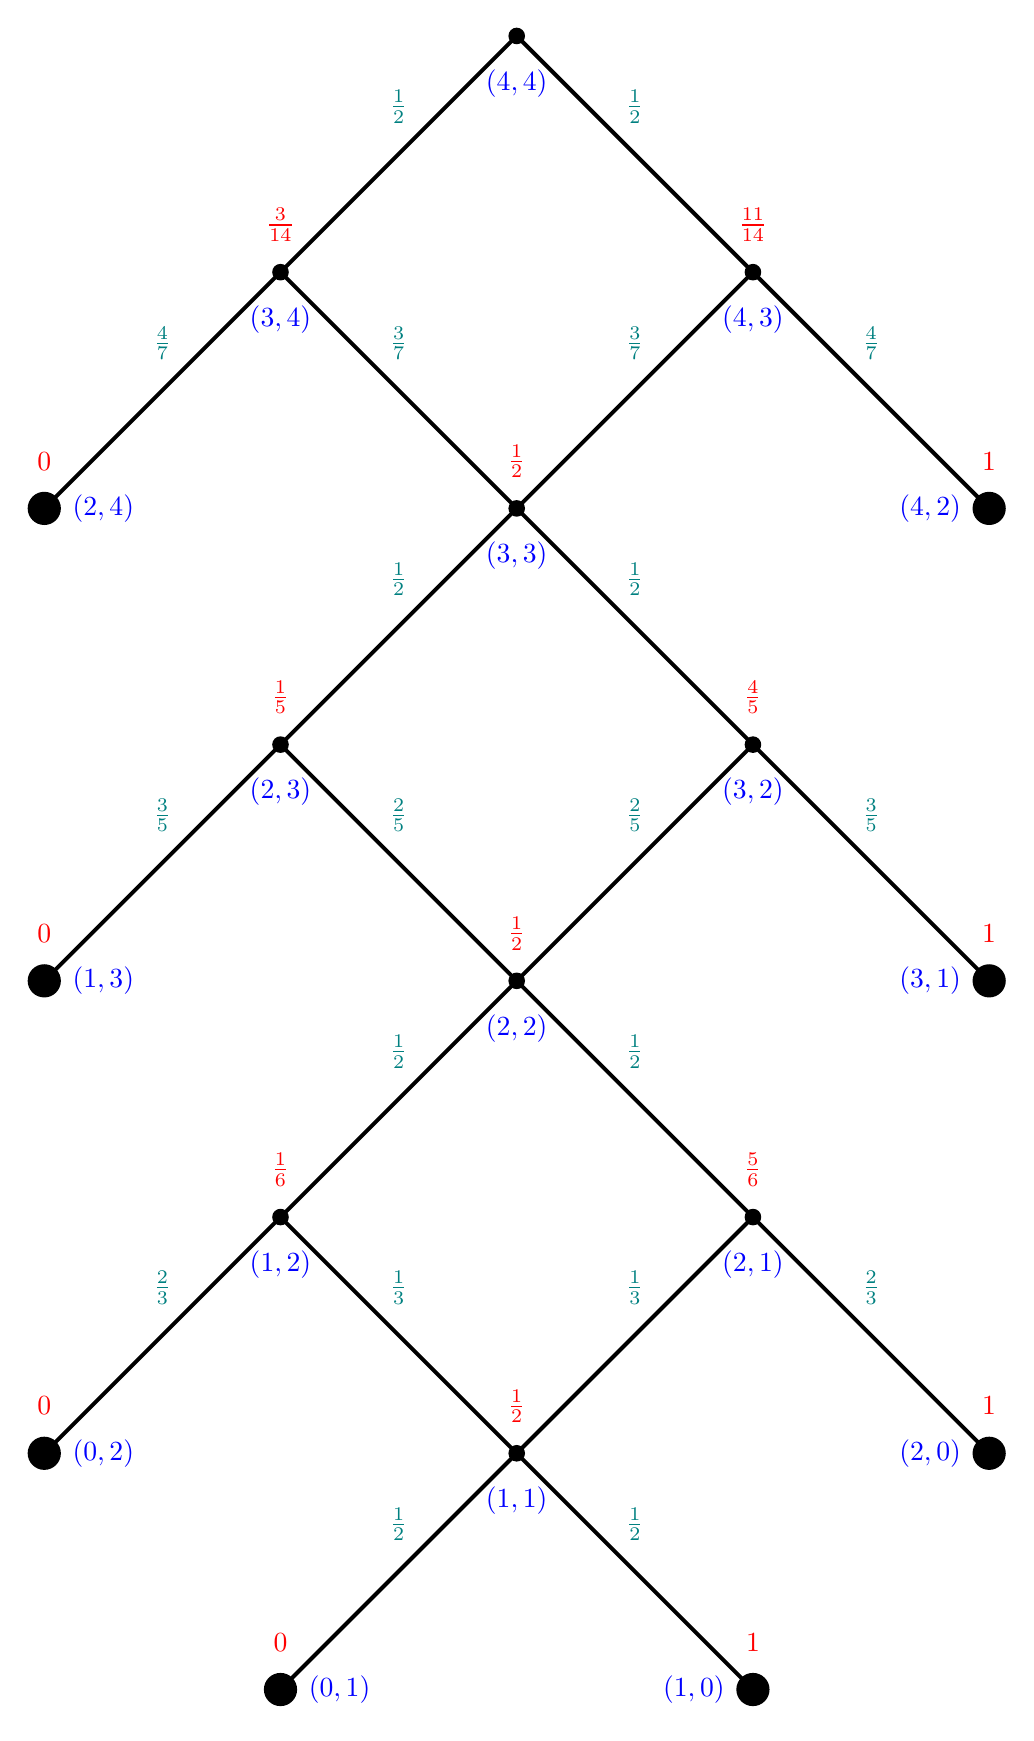
\begin{tikzpicture}[line cap=round,line join=round,x=3cm,y=3cm]


\node[text=red ] at (-1.0, 0.2)  {$0$};
\node[text=red ] at ( 1.0, 0.2)  {$1$};
\node[text=red ] at (-2   , 1.2) {$0$};
\node[text=red ] at (-1   , 2.2) {$\frac{1}{6}$};
\node[text=red ] at ( 0   , 1.2) {\half};
\node[text=red ] at ( 1   , 2.2) {$\frac{5}{6}$};
\node[text=red ] at ( 2   , 1.2) {$1$};
\node[text=red ] at (-2   , 3.2) {$0$};
\node[text=red ] at ( 0   , 3.2) {\half};
\node[text=red ] at ( 2   , 3.2) {$1$};
\node[text=red ] at (-1   , 4.2) {$\frac{1}{5}$};
\node[text=red ] at ( 1   , 4.2) {$\frac{4}{5}$};
\node[text=red ] at (-2   , 5.2) {$0$};
\node[text=red ] at ( 0   , 5.2) {\half};
\node[text=red ] at ( 2   , 5.2) {$1$};
\node[text=red ] at (-1   , 6.2) {$\frac{3}{14}$};
\node[text=red ] at ( 1   , 6.2) {$\frac{11}{14}$};

\node[text=blue] at (-0.75,0  ) {$(0,1)$};
\node[text=blue] at ( 0.75,0  ) {$(1,0)$};
\node[text=blue] at ( 0  , 0.8) {$(1,1)$};
\node[text=blue] at (-1.75, 1.0) {$(0,2)$};
\node[text=blue] at (-1   , 1.8) {$(1,2)$};
\node[text=blue] at ( 0.0 , 2.8) {$(2,2)$};
\node[text=blue] at ( 1   , 1.8) {$(2,1)$};
\node[text=blue] at ( 1.75, 1.0) {$(2,0)$};
\node[text=blue] at (-1.75, 3.0) {$(1,3)$};
\node[text=blue] at ( 1.75, 3.0) {$(3,1)$};
\node[text=blue] at (-1   , 3.8) {$(2,3)$};
\node[text=blue] at ( 1   , 3.8) {$(3,2)$};
\node[text=blue] at ( 0.0 , 4.8) {$(3,3)$};
\node[text=blue] at (-1.75, 5.0) {$(2,4)$};
\node[text=blue] at ( 1.75, 5.0) {$(4,2)$};
\node[text=blue] at (-1   , 5.8) {$(3,4)$};
\node[text=blue] at ( 1   , 5.8) {$(4,3)$};
\node[text=blue] at ( 0.0 , 6.8) {$(4,4)$};

\node[text=teal] at (-0.5, 0.7) {\half};
\node[text=teal] at ( 0.5, 0.7) {\half};
\node[text=teal] at (-1.5 , 1.7) {$\frac{2}{3}$};
\node[text=teal] at (-0.5 , 1.7) {$\frac{1}{3}$};
\node[text=teal] at ( 0.5 , 1.7) {$\frac{1}{3}$};
\node[text=teal] at ( 1.5 , 1.7) {$\frac{2}{3}$};
\node[text=teal] at (-0.5 , 2.7) {\half};
\node[text=teal] at ( 0.5 , 2.7) {\half};
\node[text=teal] at (-1.5 , 3.7) {$\frac{3}{5}$};
\node[text=teal] at (-0.5 , 3.7) {$\frac{2}{5}$};
\node[text=teal] at ( 0.5 , 3.7) {$\frac{2}{5}$};
\node[text=teal] at ( 1.5 , 3.7) {$\frac{3}{5}$};
\node[text=teal] at (-0.5 , 4.7) {\half};
\node[text=teal] at ( 0.5 , 4.7) {\half};
\node[text=teal] at (-1.5 , 5.7) {$\frac{4}{7}$};
\node[text=teal] at (-0.5 , 5.7) {$\frac{3}{7}$};
\node[text=teal] at ( 0.5 , 5.7) {$\frac{3}{7}$};
\node[text=teal] at ( 1.5 , 5.7) {$\frac{4}{7}$};
\node[text=teal] at (-0.5 , 6.7) {\half};
\node[text=teal] at ( 0.5 , 6.7) {\half};


\draw[line width=0.5mm] ( 1,2) -- ( 0,1) node[sloped, pos=0.5, allow upside down]{\arrowIn};
\draw[line width=0.5mm] ( 1,2) -- ( 2,1) node[sloped, pos=0.5, allow upside down]{\arrowIn};
\draw[line width=0.5mm] (-1,2) -- ( 0,1) node[sloped, pos=0.5, allow upside down]{\arrowIn};
\draw[line width=0.5mm] (-1,2) -- (-2,1) node[sloped, pos=0.5, allow upside down]{\arrowIn};
\draw[line width=0.5mm] ( 0,3) -- ( 1,2) node[sloped, pos=0.5, allow upside down]{\arrowIn};
\draw[line width=0.5mm] ( 0,3) -- (-1,2) node[sloped, pos=0.5, allow upside down]{\arrowIn};
\draw[line width=0.5mm] ( 0,1) -- ( 1,0) node[sloped, pos=0.5, allow upside down]{\arrowIn};
\draw[line width=0.5mm] ( 0,1) -- (-1,0) node[sloped, pos=0.5, allow upside down]{\arrowIn};
\draw[line width=0.5mm] ( 1,4) -- ( 0,3) node[sloped, pos=0.5, allow upside down]{\arrowIn};
\draw[line width=0.5mm] ( 1,4) -- ( 2,3) node[sloped, pos=0.5, allow upside down]{\arrowIn};
\draw[line width=0.5mm] (-1,4) -- ( 0,3) node[sloped, pos=0.5, allow upside down]{\arrowIn};
\draw[line width=0.5mm] (-1,4) -- (-2,3) node[sloped, pos=0.5, allow upside down]{\arrowIn};
\draw[line width=0.5mm] ( 0,5) -- ( 1,4) node[sloped, pos=0.5, allow upside down]{\arrowIn};
\draw[line width=0.5mm] ( 0,5) -- (-1,4) node[sloped, pos=0.5, allow upside down]{\arrowIn};
\draw[line width=0.5mm] ( 1,6) -- ( 0,5) node[sloped, pos=0.5, allow upside down]{\arrowIn};
\draw[line width=0.5mm] ( 1,6) -- ( 2,5) node[sloped, pos=0.5, allow upside down]{\arrowIn};
\draw[line width=0.5mm] (-1,6) -- ( 0,5) node[sloped, pos=0.5, allow upside down]{\arrowIn};
\draw[line width=0.5mm] (-1,6) -- (-2,5) node[sloped, pos=0.5, allow upside down]{\arrowIn};
\draw[line width=0.5mm] ( 0,7) -- ( 1,6) node[sloped, pos=0.5, allow upside down]{\arrowIn};
\draw[line width=0.5mm] ( 0,7) -- (-1,6) node[sloped, pos=0.5, allow upside down]{\arrowIn};

\fill ( 1,0) circle[radius=6pt];
\fill (-1,0) circle[radius=6pt];
\fill (-2,1) circle[radius=6pt];
\fill ( 0,1) circle[radius=3pt];
\fill ( 2,1) circle[radius=6pt];
\fill (-1,2) circle[radius=3pt];
\fill ( 1,2) circle[radius=3pt];
\fill (-2,3) circle[radius=6pt];
\fill ( 0,3) circle[radius=3pt];
\fill ( 2,3) circle[radius=6pt];
\fill (-1,4) circle[radius=3pt];
\fill ( 1,4) circle[radius=3pt];
\fill (-2,5) circle[radius=6pt];
\fill ( 0,5) circle[radius=3pt];
\fill ( 2,5) circle[radius=6pt];
\fill (-1,6) circle[radius=3pt];
\fill ( 1,6) circle[radius=3pt];
\fill ( 0,7) circle[radius=3pt];
\end{tikzpicture}
